\frame
{
    \frametitle{Trie}
    \framesubtitle{Properties}
    \begin{itemize}[<+->]
        \item \textless Re\emph{trie}val (but can be pronounce as either \emph{tree} or \emph{try})
        \item Store a set of words (with or without associated values)
        \item insert/retrieve in $ O(S) $, with S the length of the string
        \item Allows for non-exact matches (\textless\textgreater ~ set/map)
    \end{itemize}
}

\frame
{
    \frametitle{Trie}
    \framesubtitle{Structure}

    \begin{itemize}[<+->]
        \item Tree structure
        \item Stores the \emph{path} for the string instead of the string
        \item Edges labeled with single characters
        \item If the last character of a stored word, marked (+ associated value)
        \item Can vary in type of \emph{character} (bits/ints/\dots)
        \item Can be compressed by eliminating successive single-edge nodes
    \end{itemize}
}

\frame
{
    \frametitle{Trie}
    \framesubtitle{Structure}

    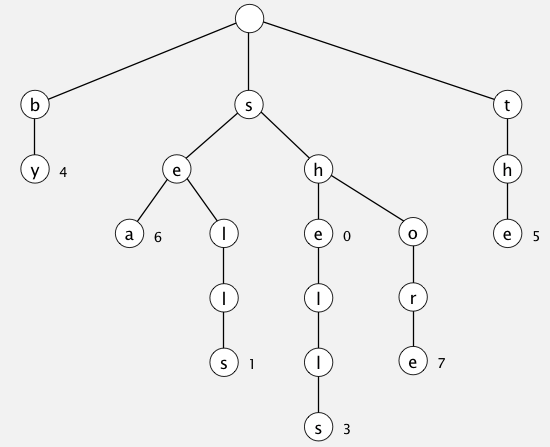
\includegraphics[width=0.8\textwidth]{img/trie.png}
}

\frame
{
    \frametitle{Trie}
    \framesubtitle{Usage}
    \begin{itemize}[<+->]
        \item Spelling suggestions
        \item Autocompletion
        \item Bioinformatics (DNA/RNA)
        \item Alphabetical ordering / sorting
        \item (Similar to structure for Aho-Corasick)
        \item (Basis for \emph{suffix tree})
    \end{itemize}
} 

\begin{frame}[fragile]
    \frametitle{Trie}
    \framesubtitle{Code}
    \lstinputlisting[language=C++,basicstyle=\tiny,keywordstyle=\color{blue},firstline=1,lastline=9]{src/trie.cpp}
\end{frame}

\begin{frame}[fragile]
    \frametitle{Trie}
    \framesubtitle{Code}
    \lstinputlisting[language=C++,basicstyle=\tiny,keywordstyle=\color{blue},firstline=11,lastline=22]{src/trie.cpp}
\end{frame}

\begin{frame}[fragile]
    \frametitle{Trie}
    \framesubtitle{Code}
    \lstinputlisting[language=C++,basicstyle=\tiny,keywordstyle=\color{blue},firstline=24,lastline=33]{src/trie.cpp}
\end{frame}
